%%%%%%%%%%%%%%%%%%%%%%%%%%%%%%%%%%%%%%%%%%%%%%%%%%%%%%%%%%%%%%%%%%%%
% Authors: A. Herrera-Poyatos, F. Herrera
% Tittle: Algoritmo memético equilibrado con diversificación voraz
% 							 CAEPIA 2015
%%%%%%%%%%%%%%%%%%%%%%%%%%%%%%%%%%%%%%%%%%%%%%%%%%%%%%%%%%%%%%%%%%%%

\section{TPCx-HS}

	\subsection*{¿Por qué usar TPCx-HS?}

		\begin{frame}{¿Qué es TPCx-HS?}
			\kern -10mm
			\begin{flushright}
					
\includegraphics[width=0.2\textwidth]{./Images/tpc-logo.png}
			\end{flushright}
			\kern -2mm
			\begin{tcolorbox}[colback=ChetwodeBlue!10,colframe=ChetwodeBlue!60]
				\fontsize{8}{8}\selectfont
				\centering
				\textbf{Transaction Processing Performance Council Express Hadoop System}
			\end{tcolorbox}

			\begin{columns}[c]
				\column{.7\textwidth}					
					\kern-2mm
					\begin{center}
						{\color{TurkishRose}\large \textbf{Benchmarking Hadoop}}						
					\end{center}
					
					\kern 3mm

					{\color{ChetwodeBlue}\large Carga de trabajo de TPCx-HS}		
					\begin{itemize}
						\fontsize{8}{10}\selectfont
						\item HSGen: generación de datos con un factor de escala.
						\item HSDataCheck: comprobación de los datos.
						\item HSSort: Implementación en Hadoop de TeraSort.
						\item HSValidate: comprobación de la salida.
					\end{itemize}		
			
				\column{.3\textwidth}
					\begin{figure}[h]
						\centering
						
\includegraphics[width=0.9\textwidth]{./Images/hardwork.png}
						
						
\includegraphics[width=0.7\textwidth]{./Images/benchmark.png}
					\end{figure}
			\end{columns}
		\end{frame}
	
	\subsection*{Funcionamiento de TPCx-HS}	

		\begin{frame}{Funcionamiento de TPCx-HS}
			\begin{tcolorbox}[colback=ChetwodeBlue!10,colframe=ChetwodeBlue!60]
				\fontsize{8}{8}\selectfont
				\centering
				\textbf{Dos ejecuciones de cinco fases cada una.}
			\end{tcolorbox}
			
				\begin{columns}[c]
					\column{.6\textwidth}
						\fontsize{8}{10}\selectfont
											
						\begin{itemize}
							\item Fase 1: Generación de los datos. \\ 3-ways replication
							\item Fase 2: Verificación de la validez de los datos.
							\item Fase 3: Ordenación de los datos.  \\ 3-ways replication
							\item Fase 4: Verificación de la validez de los datos.
							\item Fase 5: Validación de la salida
						\end{itemize}
					
					\column{.4\textwidth}
						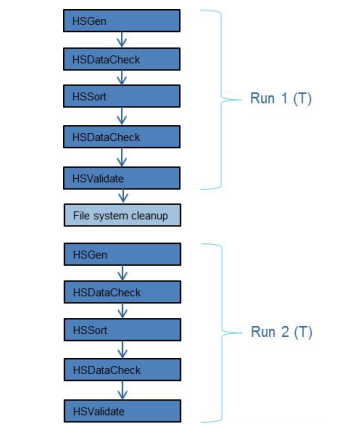
\includegraphics[width=\textwidth]{./Images/executionsTPC.png}
				\end{columns}
	
		\end{frame}
		
	\subsection*{Medida del rendimiento}	
			
		\begin{frame}{Rendimiento}		
			
			{\color{ChetwodeBlue}\large Medida del rendimiento.}
								
					$$ HSph@SF = \frac{SF}{T/3600} $$				
				
			{\color{ChetwodeBlue}\large Medida del rendimiento-precio.}
			
					$$ \$/HSph@SF = \frac{P}{HSph@SF} $$
					
			\begin{tcolorbox}[colback=blue!5,colframe=blue!15]
				\textbf{Parámetros:}
		
				\begin{itemize}
					\fontsize{10}{10}\selectfont
					\item SF: factor de escala escogido.
					\item T: tiempo total de las dos ejecuciones.
					\item P: costo del sistema bajo estudio.
				\end{itemize}
			\end{tcolorbox}
		\end{frame}
				 